\section{Sample Preparation}

The isotopic Sn samples were prepared by melting isotopically-enriched foils to
800 C in a tube furnace, cooling to ambient temperature, and pressing to the
desired shape in a tempered die. To reduce formation of tin
oxide during melting, the samples were placed in a vitreous carbon crucible
and kept under a reducing atmosphere (90\% Argon/ 10\%H2) while at elevated
temperatures. Of the 4.9 grams of \snTwelve used to prepare the sample,
3.5 grams were from
semi-permanent loan from the [INSERT GROUP NAME] from LBNL and the remaining
Sn112 purchased from [ISOTOPE MANUFACTURER]. All of the 5.8 grams of \snFour were purchased from
[ISOTOPE MANUFACTURER]. The natural Sn sample was prepared by melting and
pressing pellets [MANUFACTURER]. Loss of isotopic material during the
manufacturing process was minimal [insert table citation] and the final 
shapes and densities of the samples are within [X\%] of the desired values.

To conduct the total cross section measurements on oxygen isotopes,
isotopically-enriched water samples were prepared (a technique also used by
\cite{Vaughn1965, Salisbury1965}; cf.  with ZnO and BeO results of \cite{Finlay1993}).
Because the natural abundance of \oSix in H$_{2}$O is >99\%, a sample of
ordinary distilled water was used to make the O16 measurement. For the O18
measurement, we used distilled water enriched to >99\% in \oEight from
[manufacturer]. Both samples were enclosed in brass vessels with very thin
(~0.001") brass endcaps, to minimize attenuation. At the temperature and
pressure of the experimental facility, the amount of dissolved gas and ions
in the water samples were small enough to have no effect on the measurement.

The natural and isotopic Ni samples were prepared by [insert name] at Oak Ridge National Lab 
(ORNL) to match the diameter of our Sn samples.

The \rhThree sample was purchased from [insert name] as four thin disks of natural Rh metal (Rh is
monoisotopic).

Lastly, two natural-abundance graphite samples of different lengths and one
natural Pb sample, all with the same diameter as the Sn and Ni samples, were
prepared by the Washington University Machine Shop. These
samples were used to benchmark the total cross sections measured at LANSCE by
comparison with previous measurements of the C and Pb total cross sections
available in the literature (\cite{Finlay1993,Abfalterer2001}. Before use any
measurement, the C samples were baked in an oven for several
hours to remove residual machining oil and water.

Except for the oxygen and rhodium samples, the final form for each sample was a right
cylinders 8.25 mm in diameter and ranging from 10-27 mm in length (see
Table \ref{SampleTable} for sample characteristics and Fig. \ref{SamplesImage}
for sample images). A natural-abundance sample
was also prepared for each element. The samples
were inserted into styrofoam sleeves and seated in the cradles of the sample
changer. This design minimizes the amount of non-target mass proximate to the
neutron beam path.

\begin{table*}[ht]
    \caption{
        Physical characteristics of all samples used for our \tot\
        measurements. For isotopically-enriched samples, the natural abundance
        of the enriched isotope and the isotopic fraction of the sample are
        given. To calculate cross sections, the relevant ``sample thickness" is the areal
        density of nuclei $\rho_{\text{areal}}$, equivalent to
        the (volumetric) density times the length of the sample. For liquid
        samples H$_{2}^{\text{nat}}$O, D$_{2}^{\text{nat}}$O, and H$_{2}^{18}$O,
        the length and diameter listed are for the interior of the vessels
        used to hold the samples and the masses given are calculated based on 
        literature values for the density of each sample at 25\textdegree{}C.
        Our samples are generally much smaller than those used in previous
        measurements; for comparison, the Ni and Sn samples used in \cite{Abfalterer2001,
        Finlay1993} had areal densities of 1.515 and 0.5475
        $\frac{mol}{cm^{2}}$, respectively (12.7 and 6.5 times larger than our
    Ni and Sn samples).}
    \label{SampleCharacteristics}
    \begin{center}
        \begin{tabular}{ c c c c c c c }
            \hline
            Isotope & Length & Diameter
            & Mass & $\rho_{\text{areal}}$ & Nat. Abund. & Sample Purity\\
                 & [mm] & [mm] & [g] & [$\frac{mol}{cm^{2}}$] & [\%] & [\%]\\
            \hline

            $^{\text{nat}}$C & 13.66(2) & 8.260(5) & 1.2363
            & 0.1921(1) & - & -\\
            $^{\text{nat}}$C & 27.29(2) & 8.260(5) & 2.4680
            & 0.3835(2) & - & -\\

            H$_{2}$$^{\text{nat}}$O & 20.00(1) & 8.92(1) & 1.2461 & 0.1107(3) & - &
            - \\
            D$_{2}$$^{\text{nat}}$O & 20.00(1) & 8.92(1) & 1.3852 & 0.1107(3) & - &
            - \\
            H$_{2}$$^{18}$O & 20.00(1) & 8.92(1) & 1.3844 & 0.1107(3) & 0.20 & 99\\

            $^{58}$Ni & 7.97(3)& 8.18(2) &
            3.6438 & 0.1197(3)& 68.1 & 99.6 \\
            $^{\text{nat}}$Ni & 8.00(3) & 8.20(2) &
            3.6898 & 0.1192(3)& - & -\\
            $^{64}$Ni & 7.96(2) & 8.20(4) &
            3.9942 & 0.1192(6) & 0.93 & 92.2\\

            $^{103}$Rh & 2.03(1) & 10.20(2) & 2.8359 & 0.02426(4) & 100 & 99.9\\

            $^{112}$Sn & 13.65(3) & 8.245(5) &
            4.9720 & 0.08332(5) & 0.97 & 99.9\\
            $^{\text{nat}}$Sn & 13.68(3) & 8.245(5) &
            5.3263 & 0.08414(5) & - & -\\
            $^{124}$Sn & 13.73(3) & 8.245(5) &
            5.5492 & 0.08399(5) & 5.79 & 99.9\\

            $^{\text{nat}}$Pb & 10.07(2) & 8.27(1) & 6.130 &
            0.05508(6) & - & -\\

            \hline
        \end{tabular}
    \end{center}
\end{table*}

\begin{figure}
    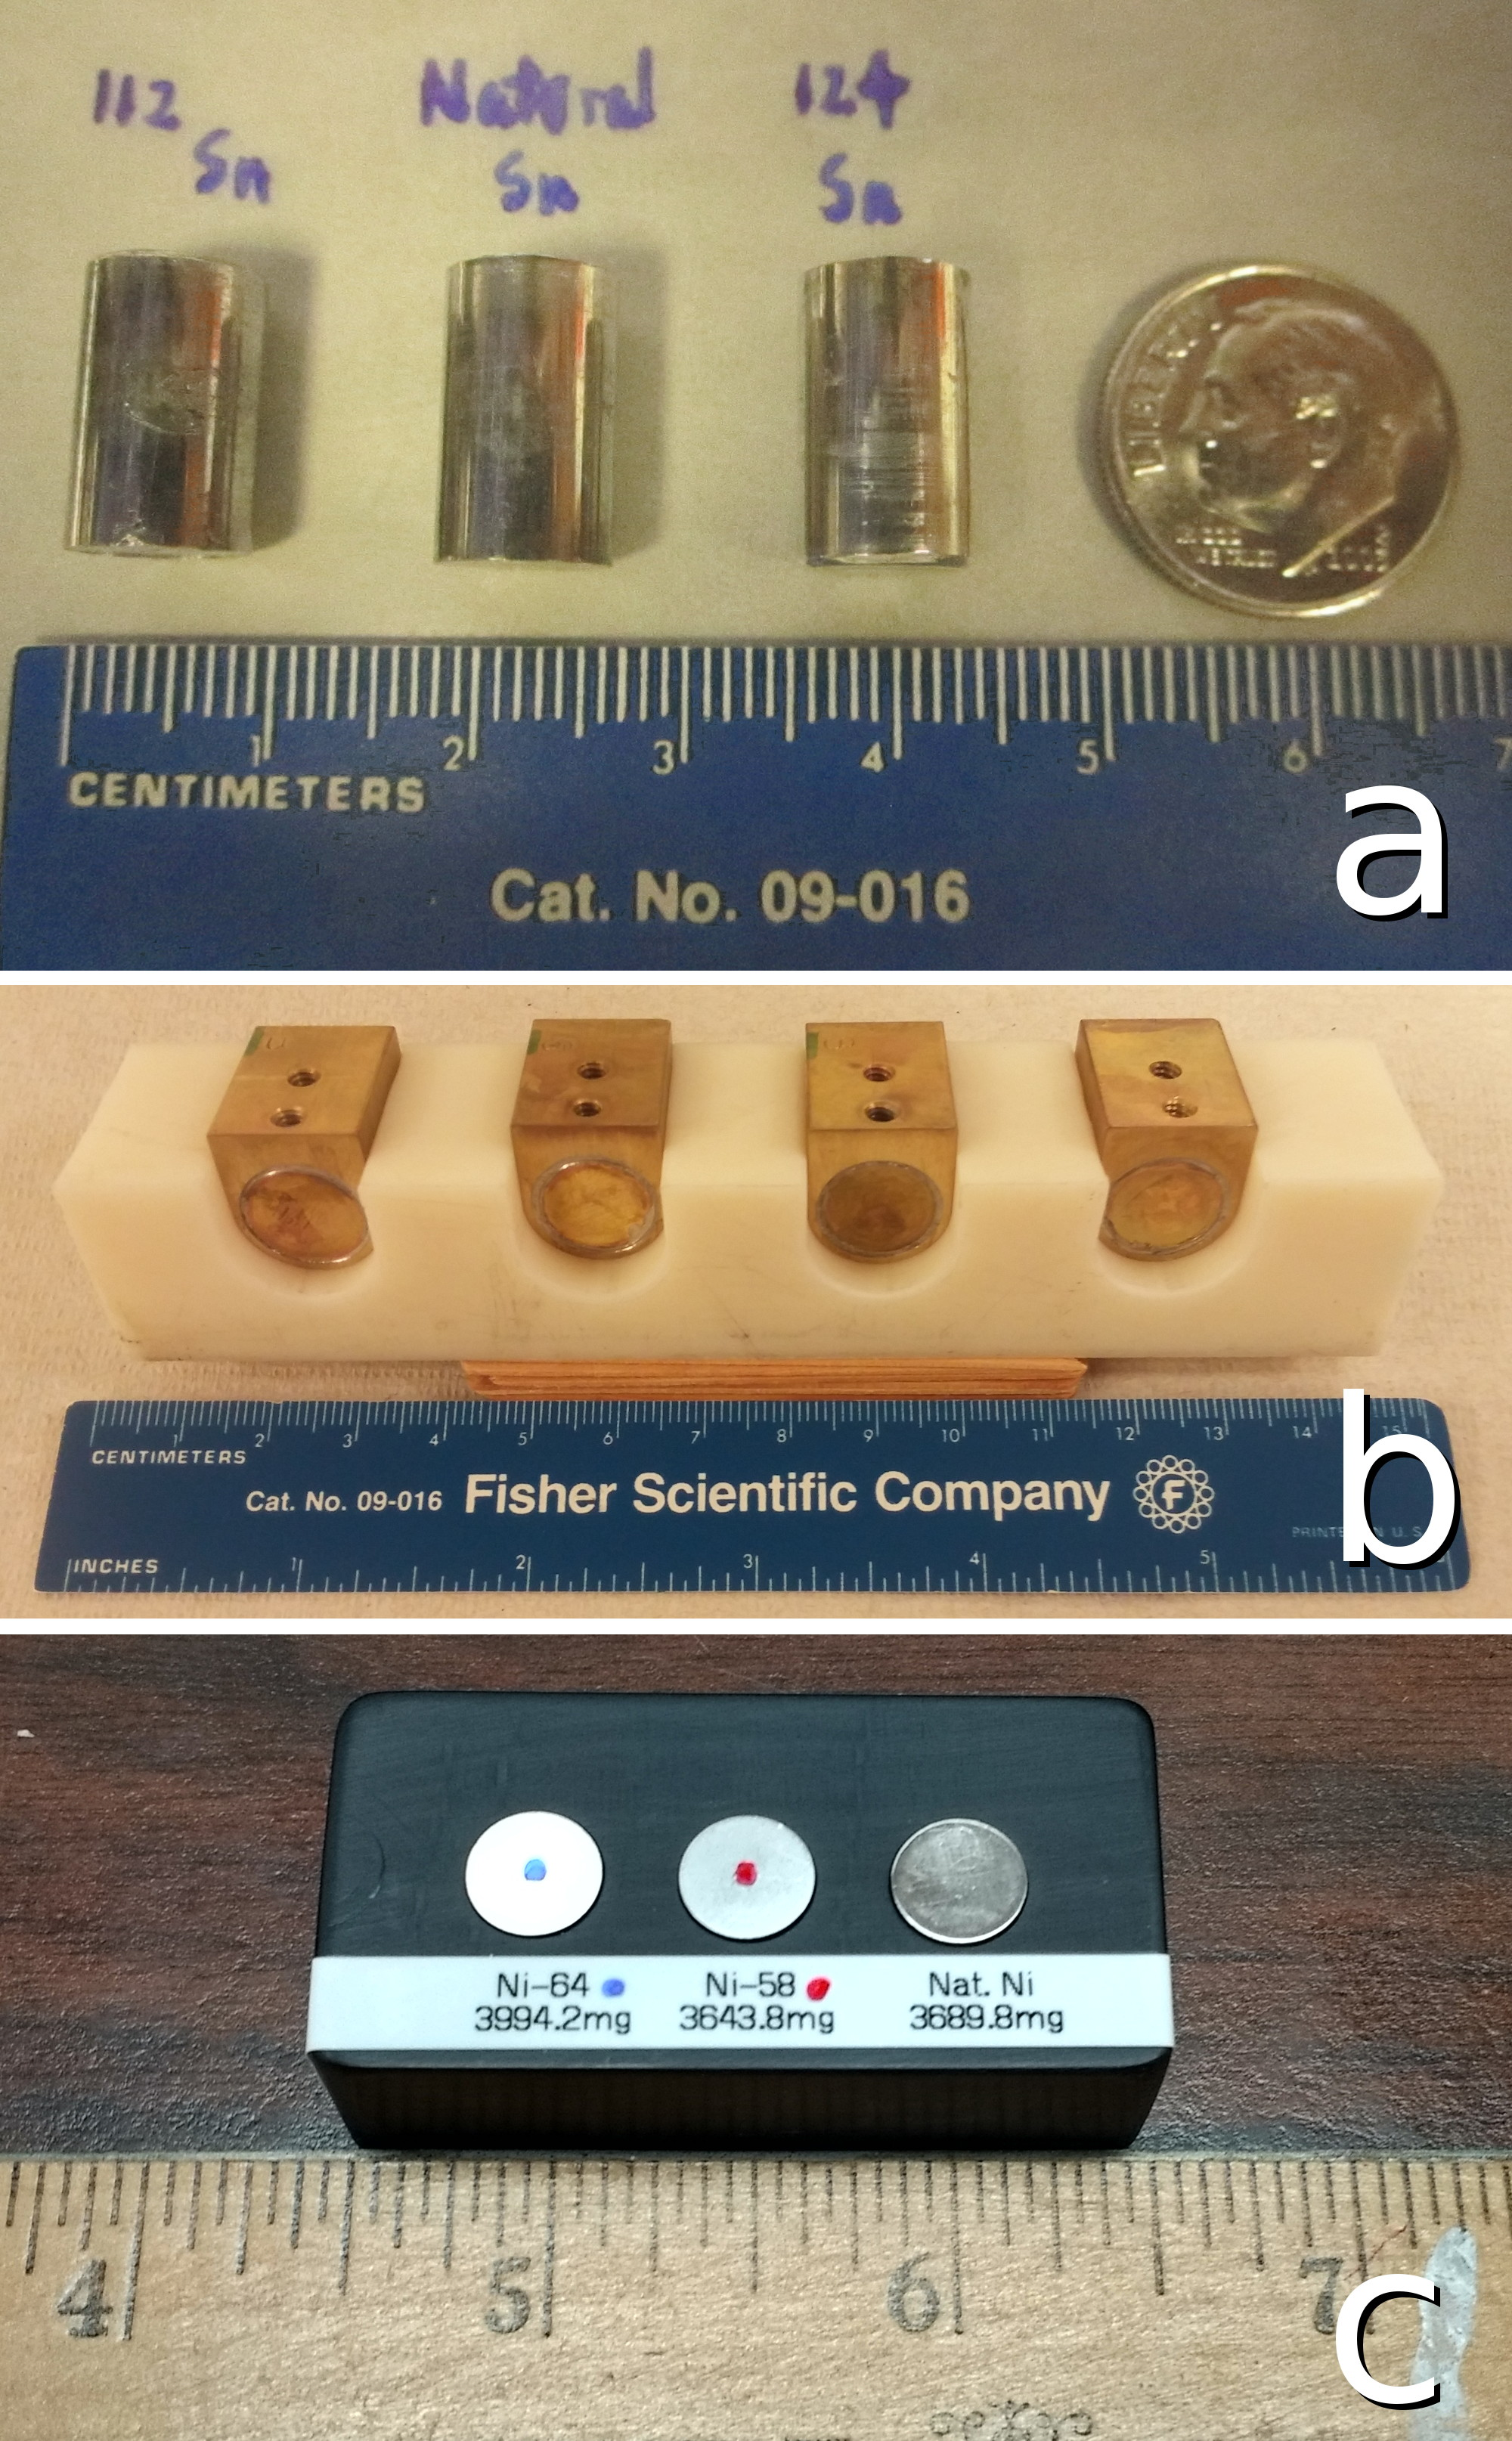
\includegraphics[scale=0.23]{figures/AllIsotopicSamples.jpg}
    \caption{${^{112,\text{nat},124}}$Sn, $^{{\text{nat}, 18}}$O, and ${^{58,\text{nat},64}}$Ni
samples used for neutron \tot measurements}
    \label{SamplesImage}
\end{figure}

\begin{figure}
    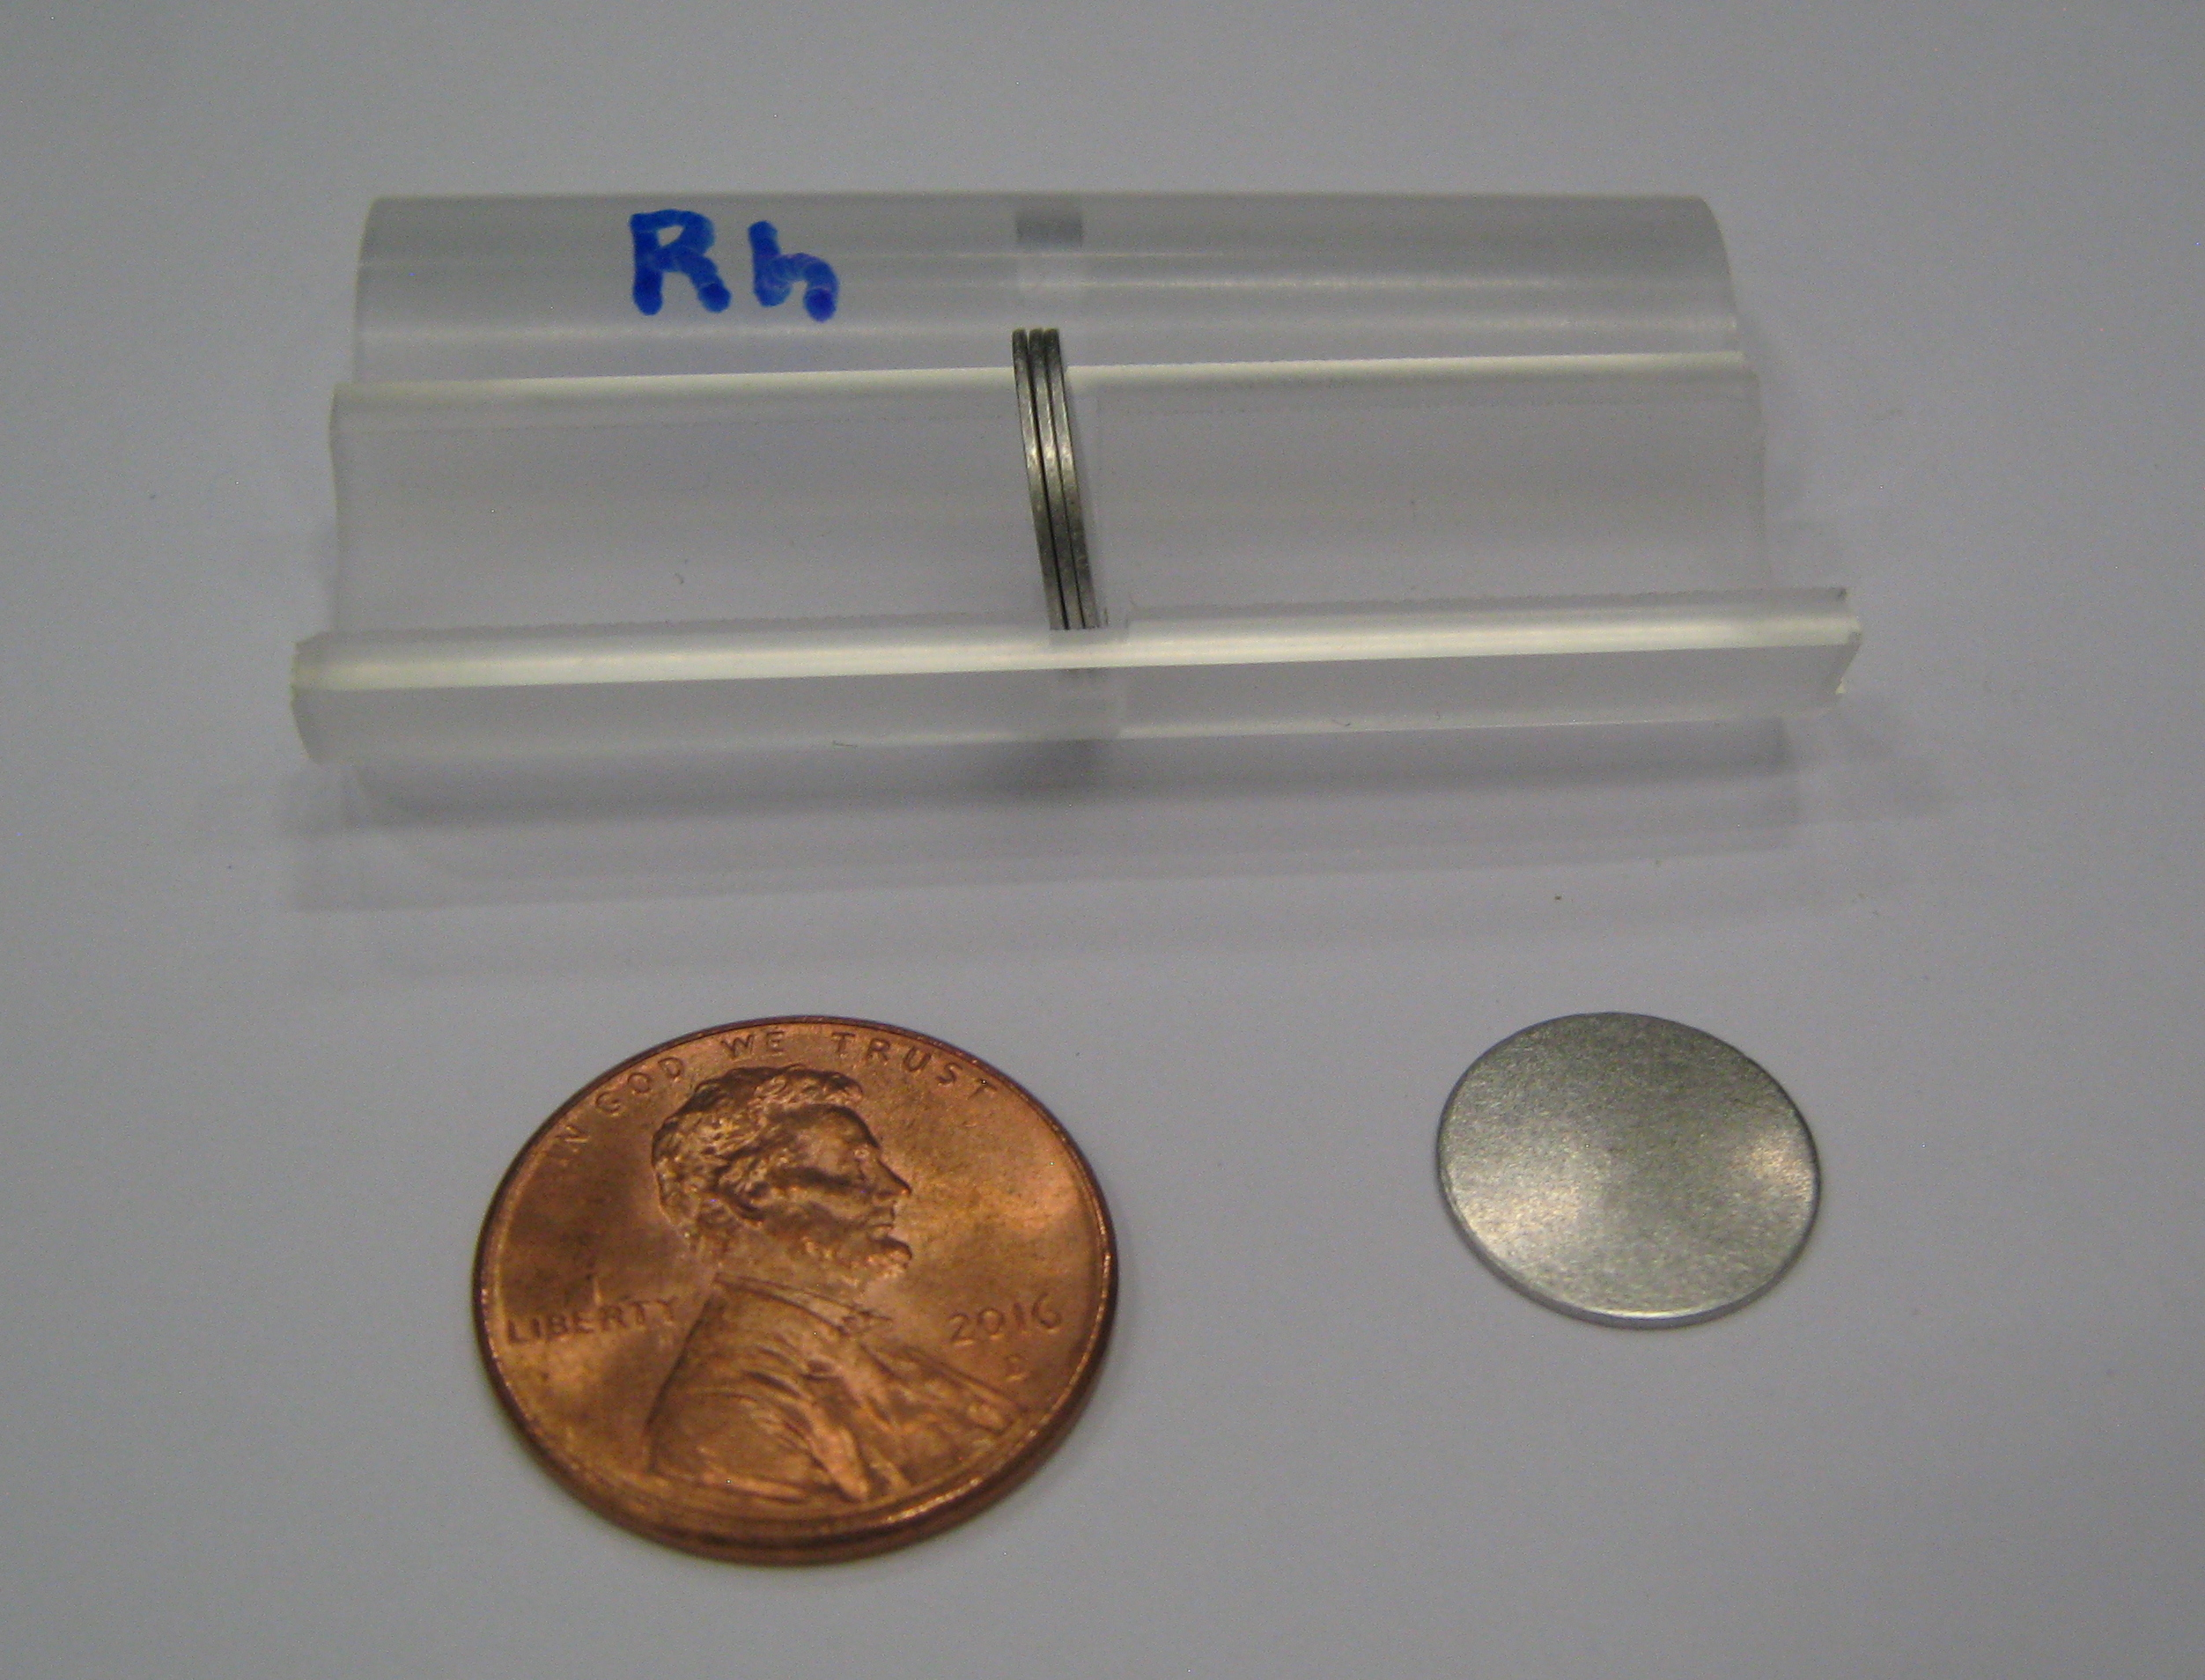
\includegraphics[scale=0.25]{figures/RhodiumSample.jpg}
    \caption{\rhThree\ sample used for the neutron \tot measurements}
    \label{SamplesImage}
\end{figure}


The oxygen isotopes were prepared as water samples to increase the areal density
of atoms and for ease of handling. Each water sample was contained by a
cylindrical brass vessel with very thin (0.002 inch) brass endcaps, minimizing
beam attenuation in the vessel. Oxygen cross sections were calculated by
subtracting the well-known hydrogen cross section from the raw H$_{2}$O result
(we used H \tot\ data sets from Clement et al \cite{Clement1972} and Abfalterer
et al \cite{Abfalterer2001}, which together cover the range $0.5 \leq E_n \leq 500$ MeV
and are in excellent agreement where their energy ranges overlap). In light of
the additional uncertainty inherent to this kind of subtractive \tot\
determination, a D$_{2}^{\text{nat}}$O sample from which the literature \tot\ for
D$_{2}$ could be subtracted was prepared as an additional cross-check. Due to its poor 
machining properties, the rhodium
sample was prepared by stacking a series of thin rhodium discs rather than by
producing a fused cylinder. These discs were contained by a cylindrical plastic
case with open ends, similar to the styrofoam sleeves.

\section{Detector Construction}
\begin{figure}
    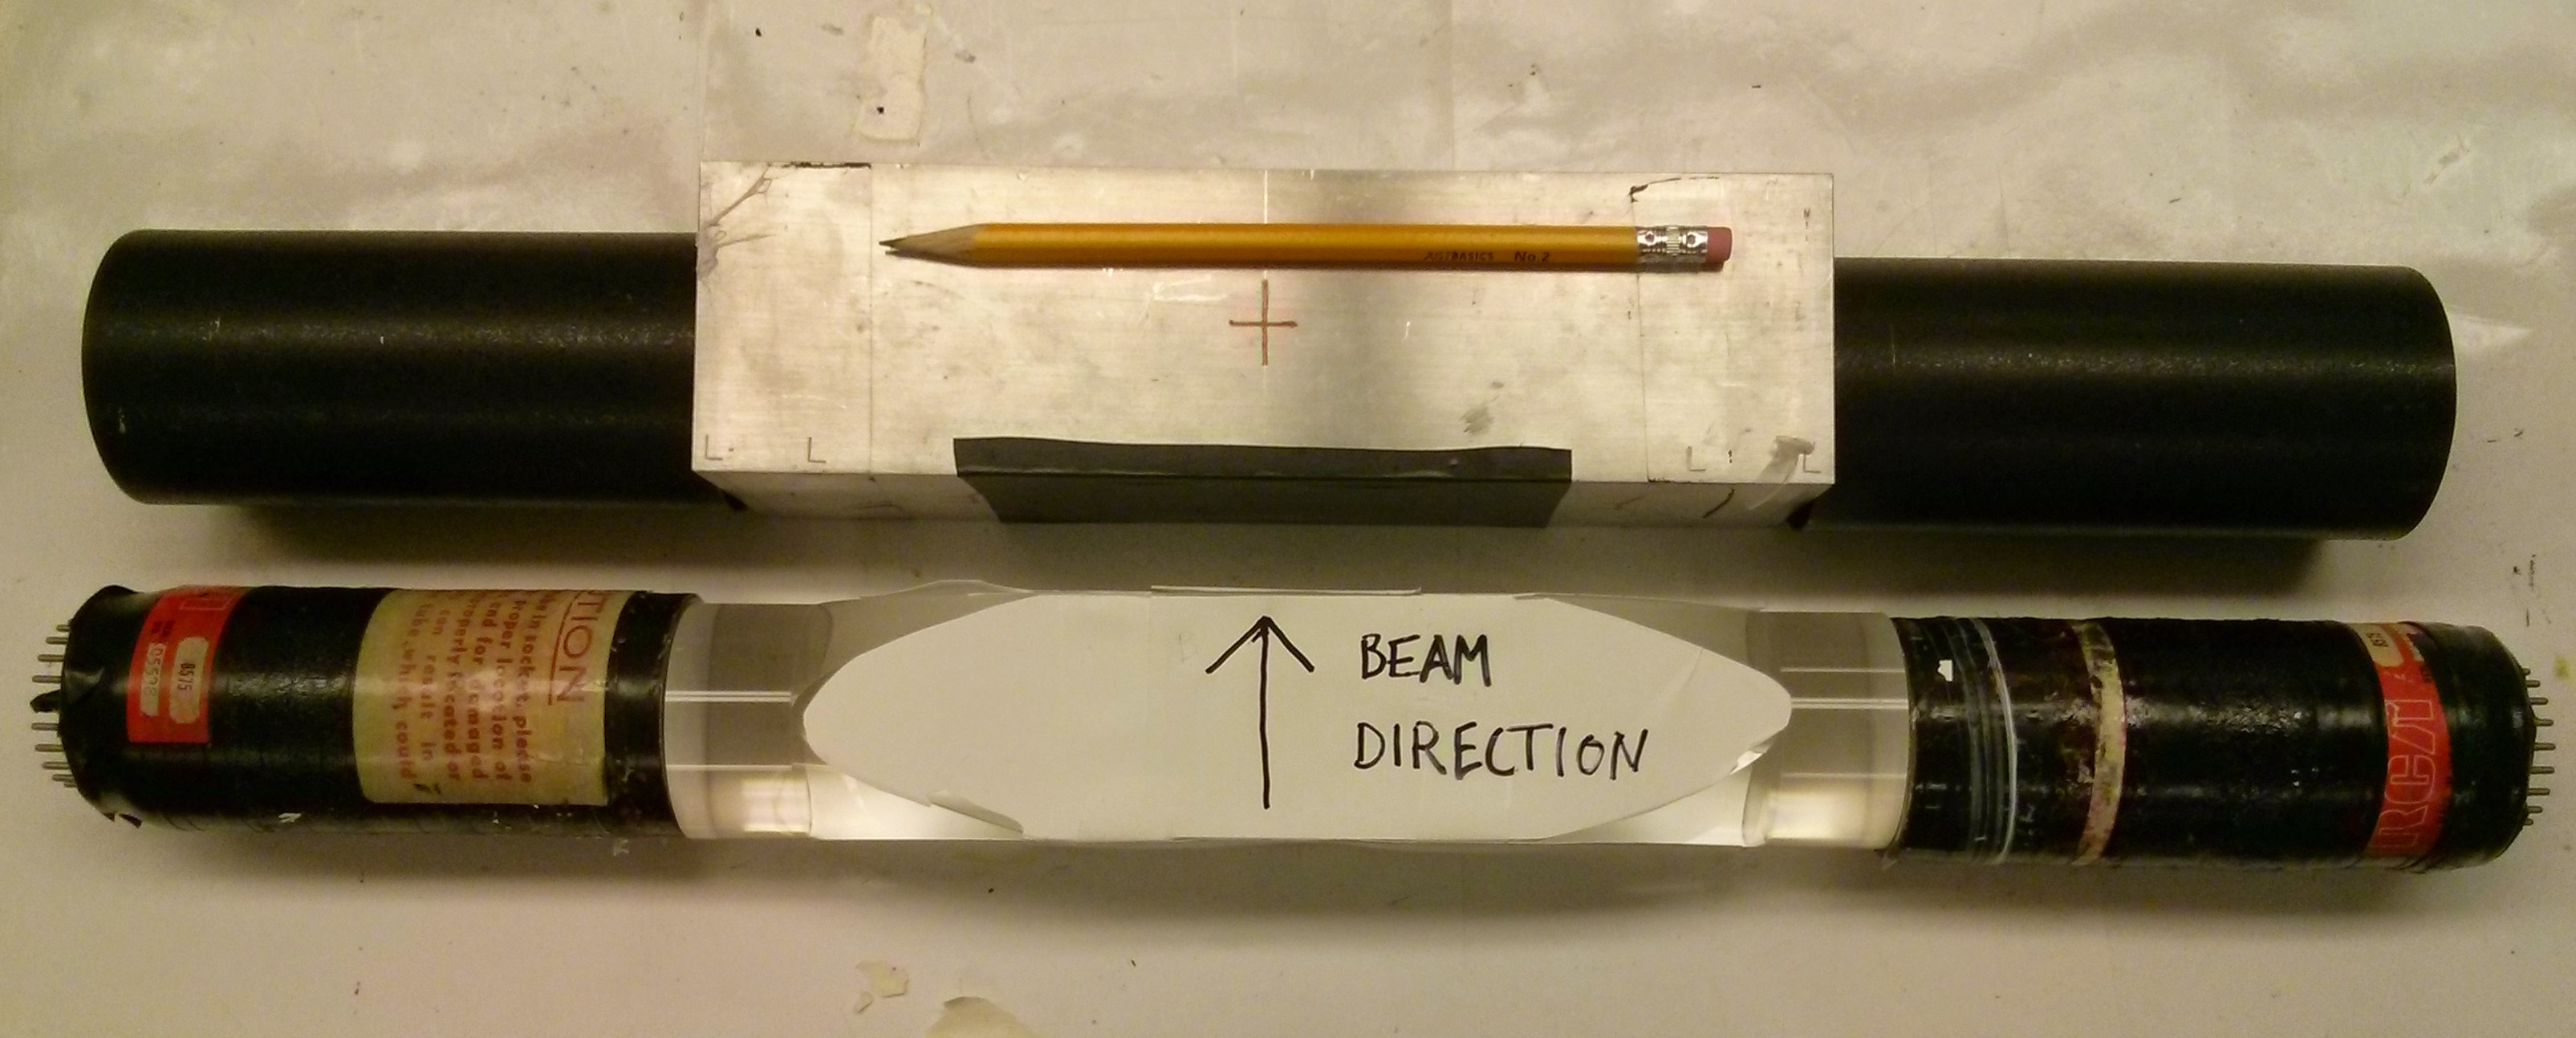
\includegraphics[scale=0.2]{figures/Scintillator_disassembled.jpg}
    \caption{The time-of-flight detector, disassembled}
    \label{TOFDetectorDisassembled}
\end{figure}

%\begin{figure}
%    \includegraphics[scale=0.6]{figures/TOFCAD.jpg}
%    \caption{CAD figure for light-tight fitting on PMT for time-of-flight detector}
%    \label{TOFCAD}
%\end{figure}

The scintillator is just under 2`` cube, so the lightguide length should be pretty close to (24
9/16'' - 2 - 2*PMT length``)/2. 

\section{Experimental Facility at LANSCE}
All neutron total cross section measurements were carried out at the 15R
beamline at the Weapons Neutron Research (WNR) facility of the Los Alamos
Neutron Science Center (LANSCE) over two run cycles (November 2016 and
September 2017). Our experiment was modeled on previous
\tot\ measurements at WNR \cite{Finlay1993,Abfalterer2001,Shane2010}. At WNR,
broad-spectrum neutrons up
to 800 MeV are generated by impinging proton pulses onto a water-cooled, 7.5
cm-long tungsten target (see Fig. \ref{ExperimentalApparatus}). Before the beam
enters the experimental area, a
permanent magnet deflects all charged particles generated by the proton pulses, 
allowing only neutrons and gamma rays to reach the flight path. Based on beam divergence
simulations, the beam was collimated to 0.200 inches using steel
donuts with a total thickness of 24 inches at the entrance to the experimental vault. To
reduce the $\gamma$-ray flux in the beam, a plug of Hevimet (90\% W, 6\% 
Ni, 4\% Cu by weight) was inserted at the upstream end of the
stack of collimator donuts. After collimation, the beam passed successively through a flux 
monitor, the sample of interest held in a sample changer, a veto detector, and finally the 
time-of-flight (TOF) detector approximately 25 meters from the neutron source.

All detectors consisted of BC-400 fast scintillating plastic mated with 
photomultiplier tubes (PMTs) and encased in a plastic or
aluminium structural housing. The flux monitor and veto detector each had
scintillator thicknesses of $\frac{1}{4}$ inch and the TOF detector had a
scintillator thickness of 1 inch. Signals from all detectors and
the target changer were relayed to a 500-MHz CAEN DT-5730 waveform digitizer
running custom software. To improve time resolution, the TOF detector used two
PMTs (one left, one right) mated to the plastic scintillator and the PMTs' signals were 
summed before digitization.

\begin{figure}
    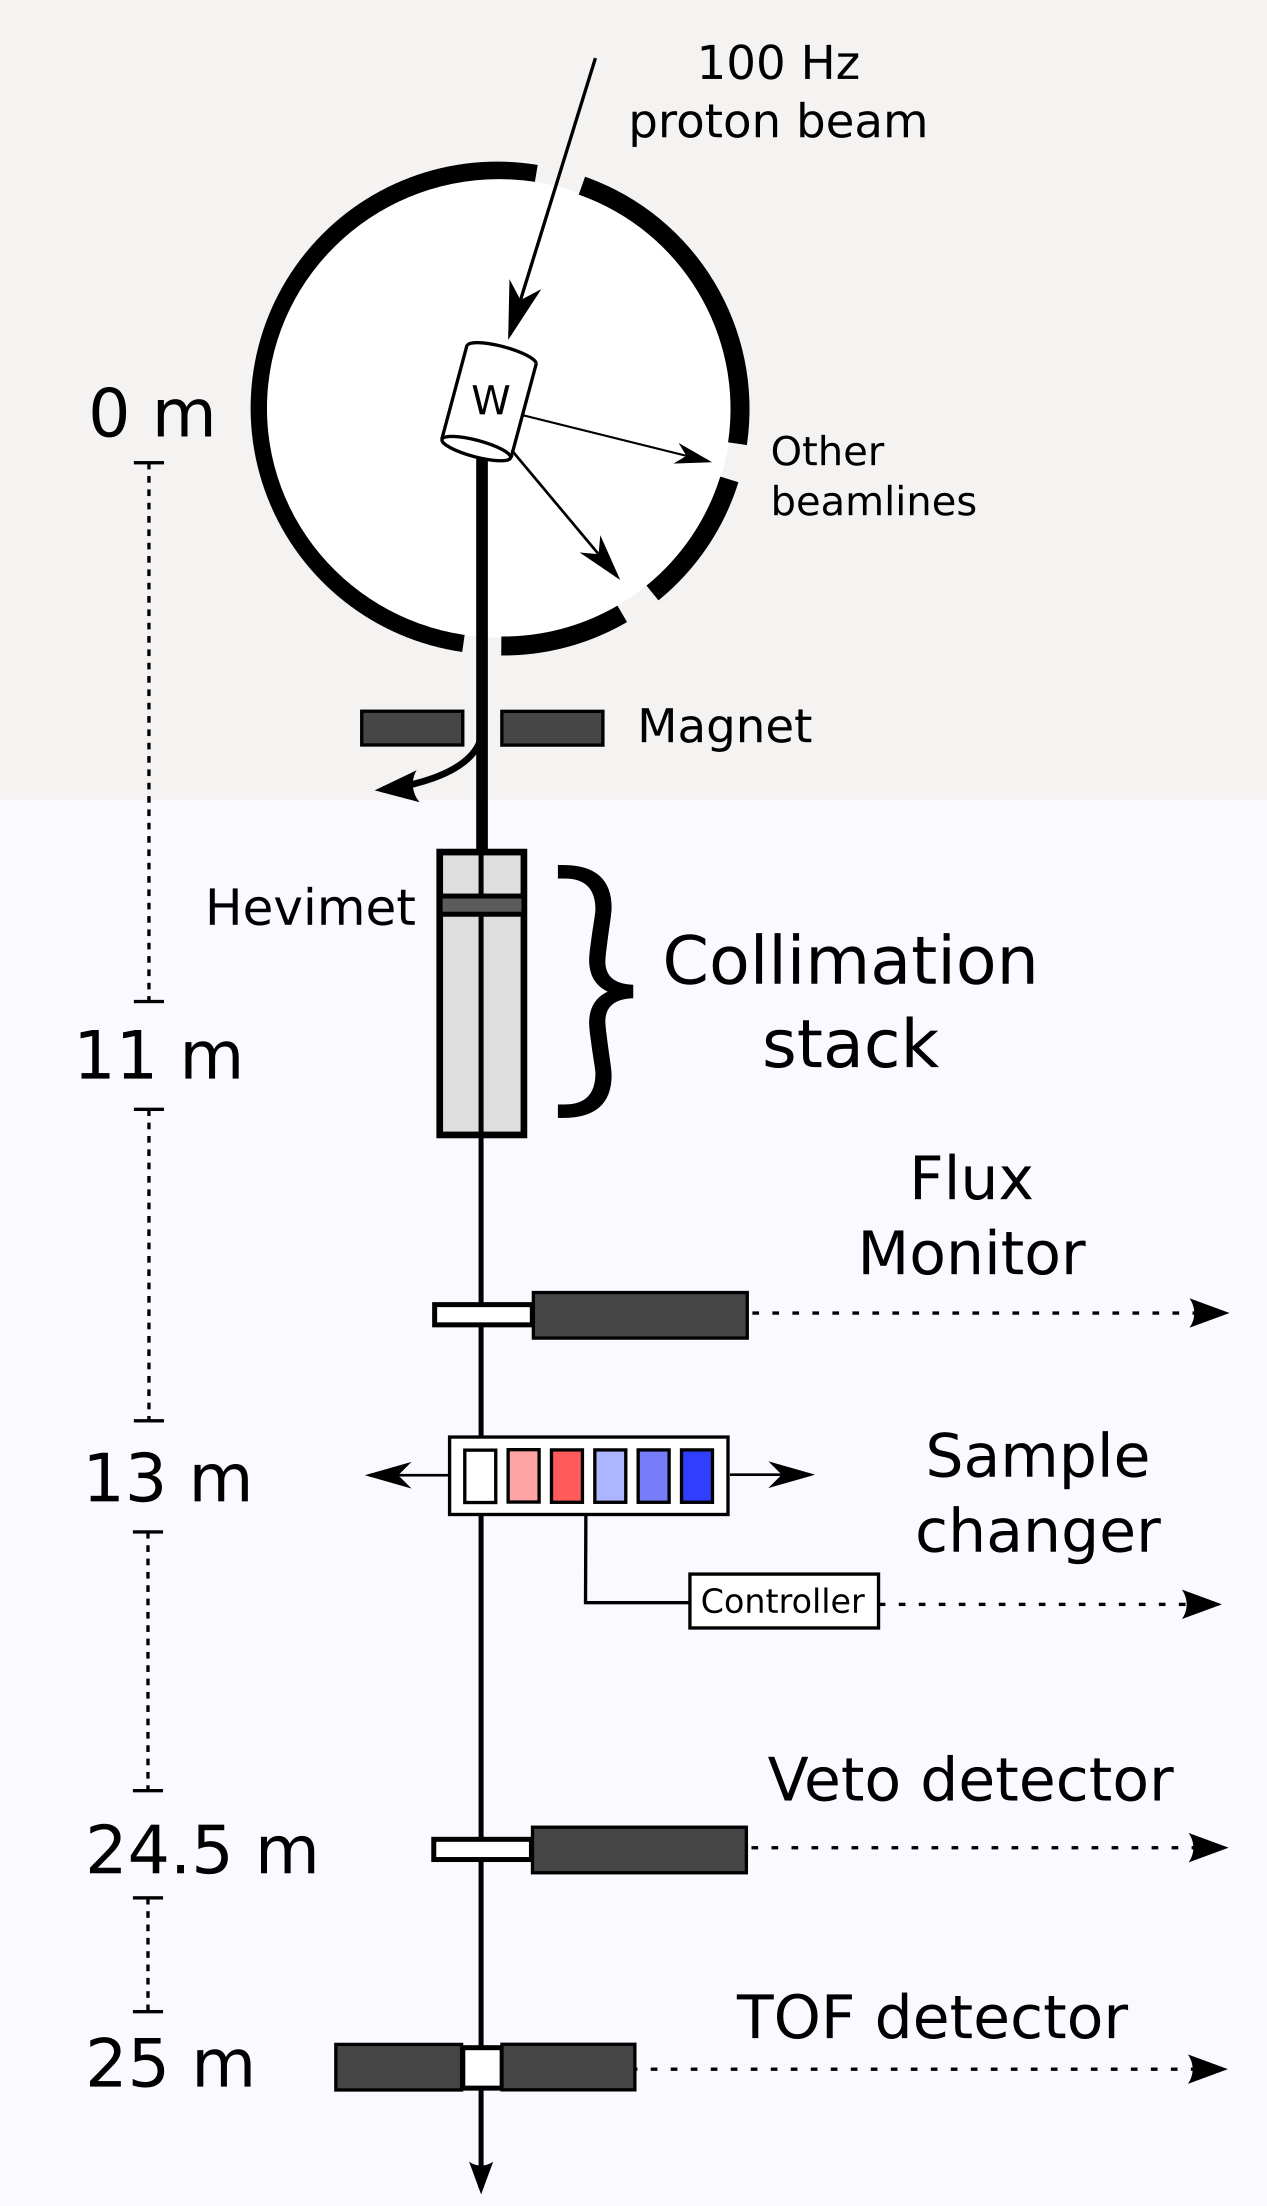
\includegraphics[scale=0.6]{figures/ExperimentalSetup.png}
    \caption{Layout of the 15R beamline at the WNR facility at LANSCE}
    \label{ExperimentalApparatus}
\end{figure}

(Color online) Experimental configuration at WNR facility. After a
        permanent magnet sweeps charged particles from the beam, neutrons and
        $\gamma$-rays are collimated to a 0.200 inch beam en route to the
        detectors used in the experiment. Samples are cycled into and out of beam
        using a linear actuator with a period of 150 seconds. Times-of-flight (TOFs) are
    determined by the TOF detector and used to calculate neutron energy.

\begin{figure*}
    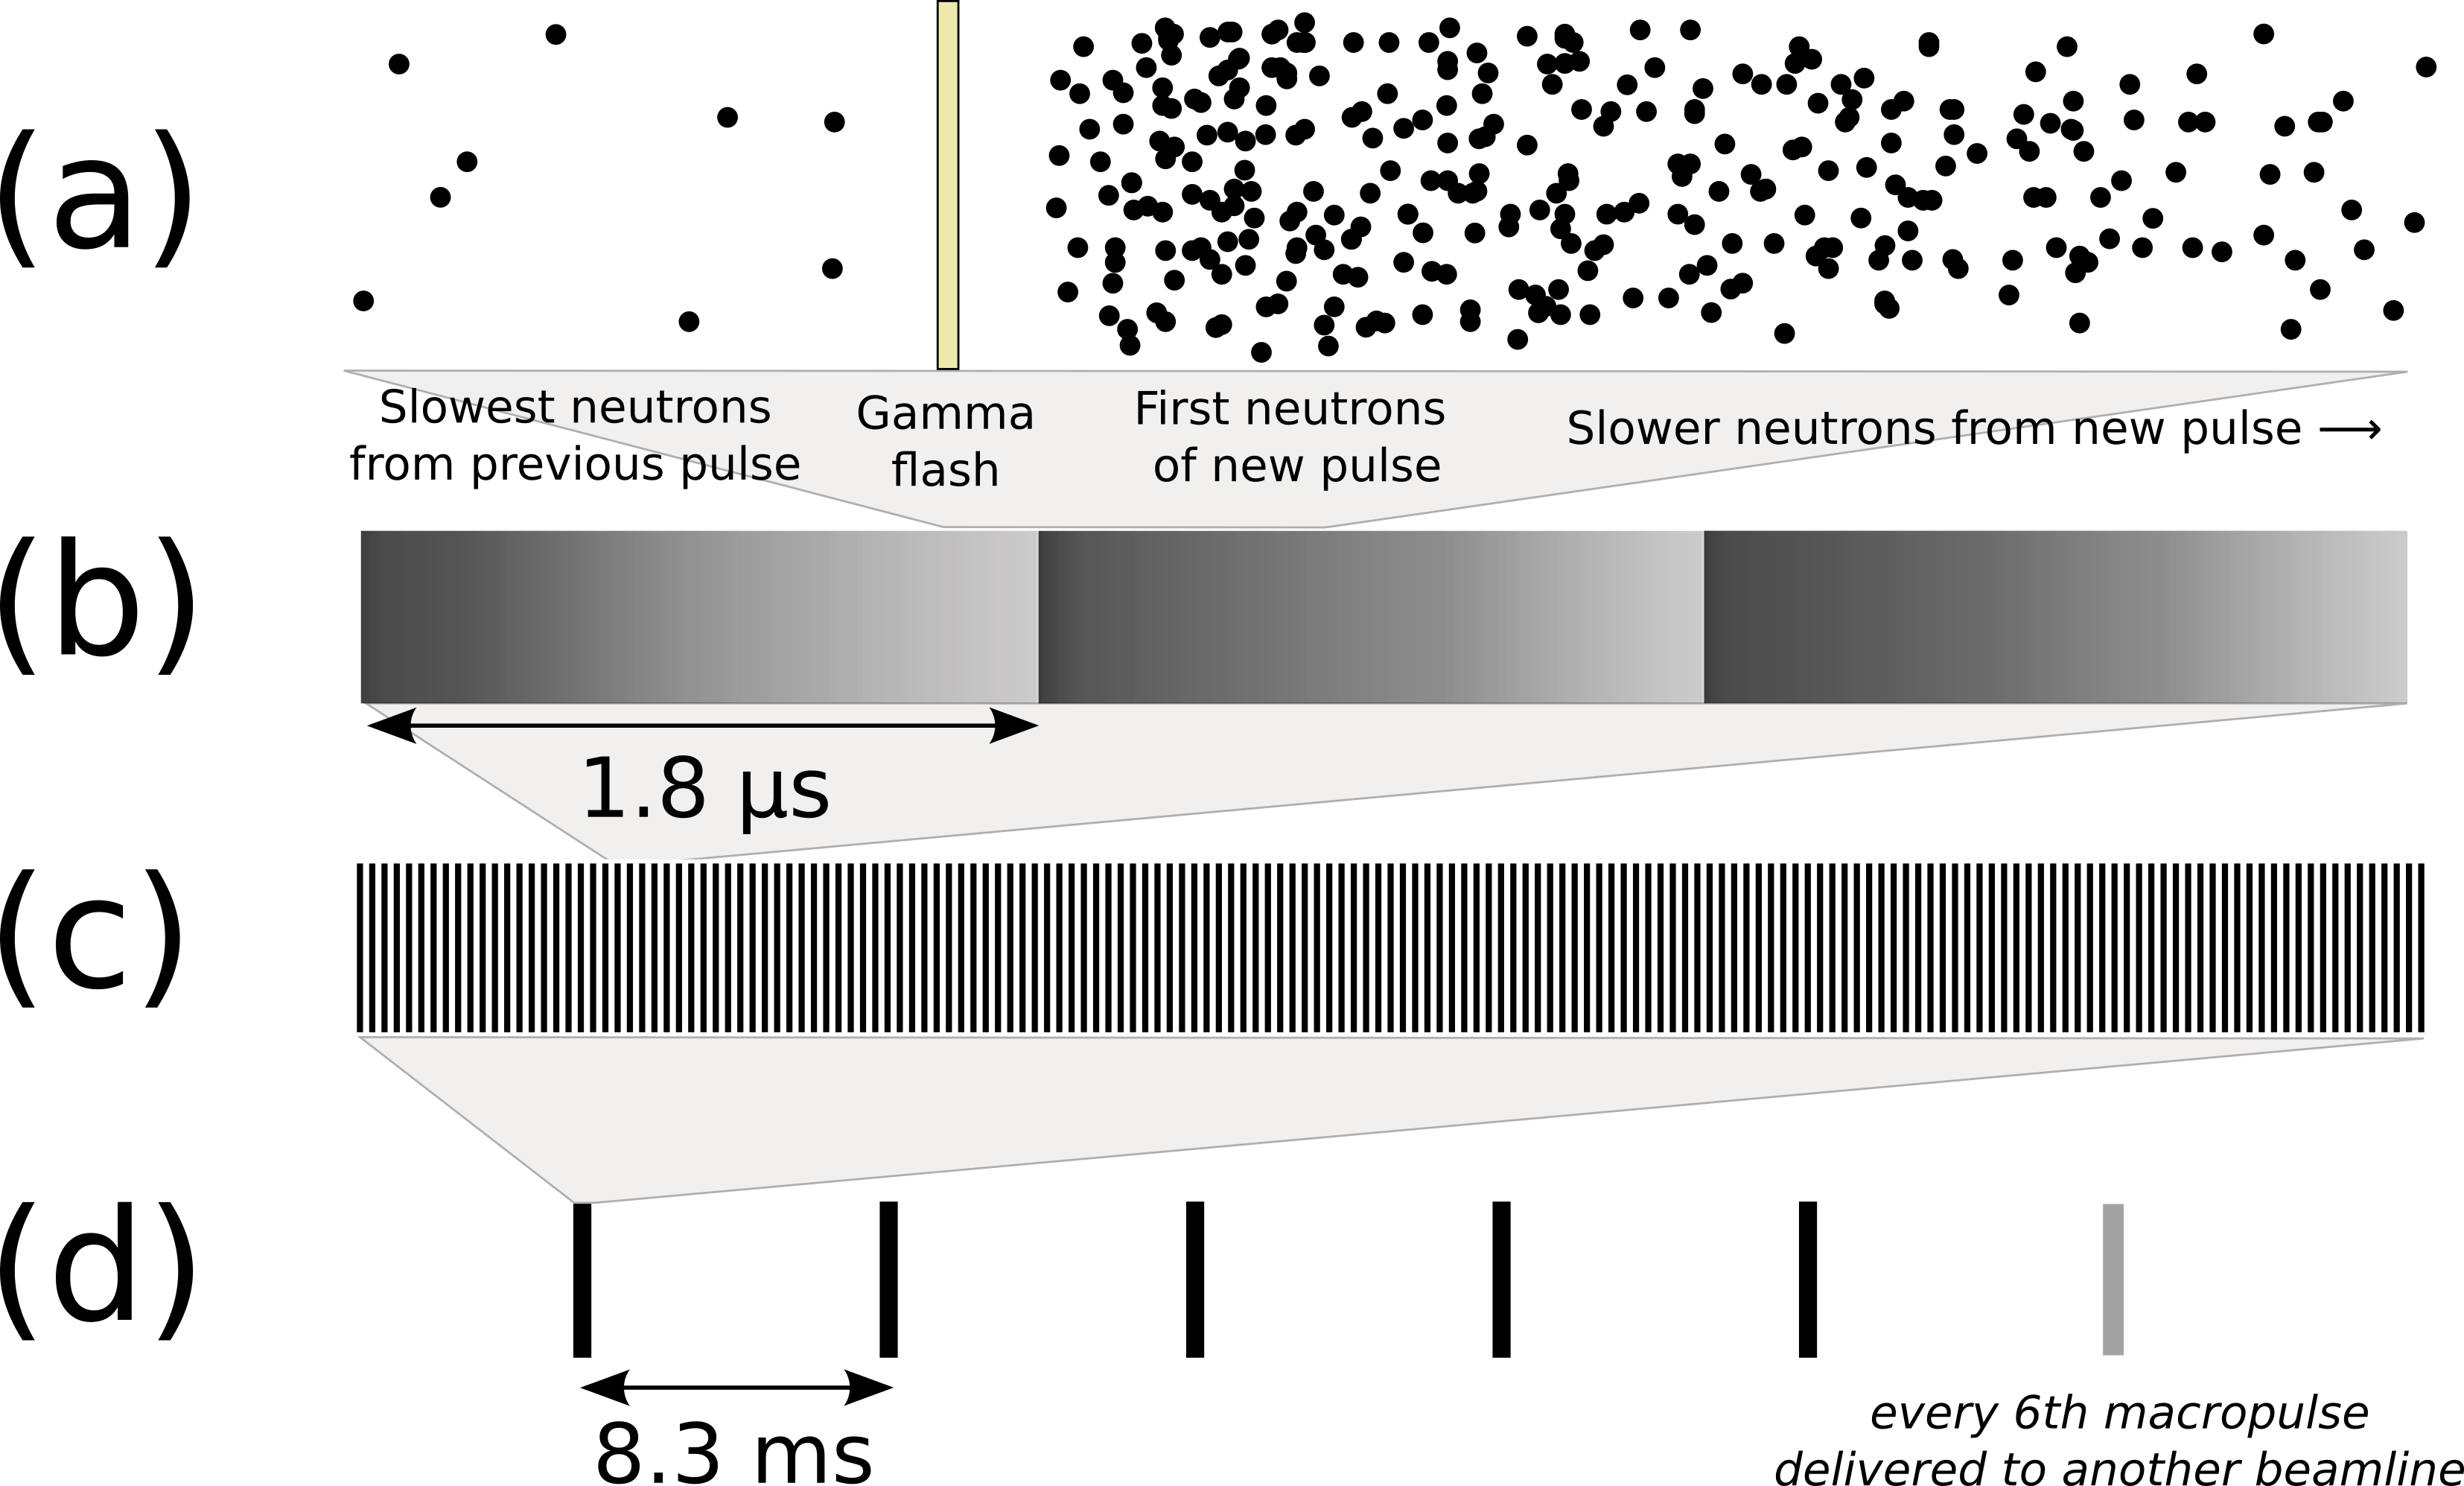
\includegraphics[scale=0.4]{figures/beamStructure.png}
    \caption{Pulsed structure of the neutron beam at the WNR facility}
    \label{BeamStructure}
\end{figure*}

(Color online) Neutron beam structure at WNR facility.
        ``Macropulses" of protons (row d) are delivered to
        WNR's tungsten Target 4, where they generate neutrons by spallation.
        Each macropulse consists of
        $\approx$350 proton ``micropulses" (row c). Neutrons
        from each micropulse (row b) disperse in
        time as they travel along the flight path so that $\gamma$ rays and high-energy 
    neutrons catch up to low-energy ones from the previous pulse (row a).

\begin{figure}
    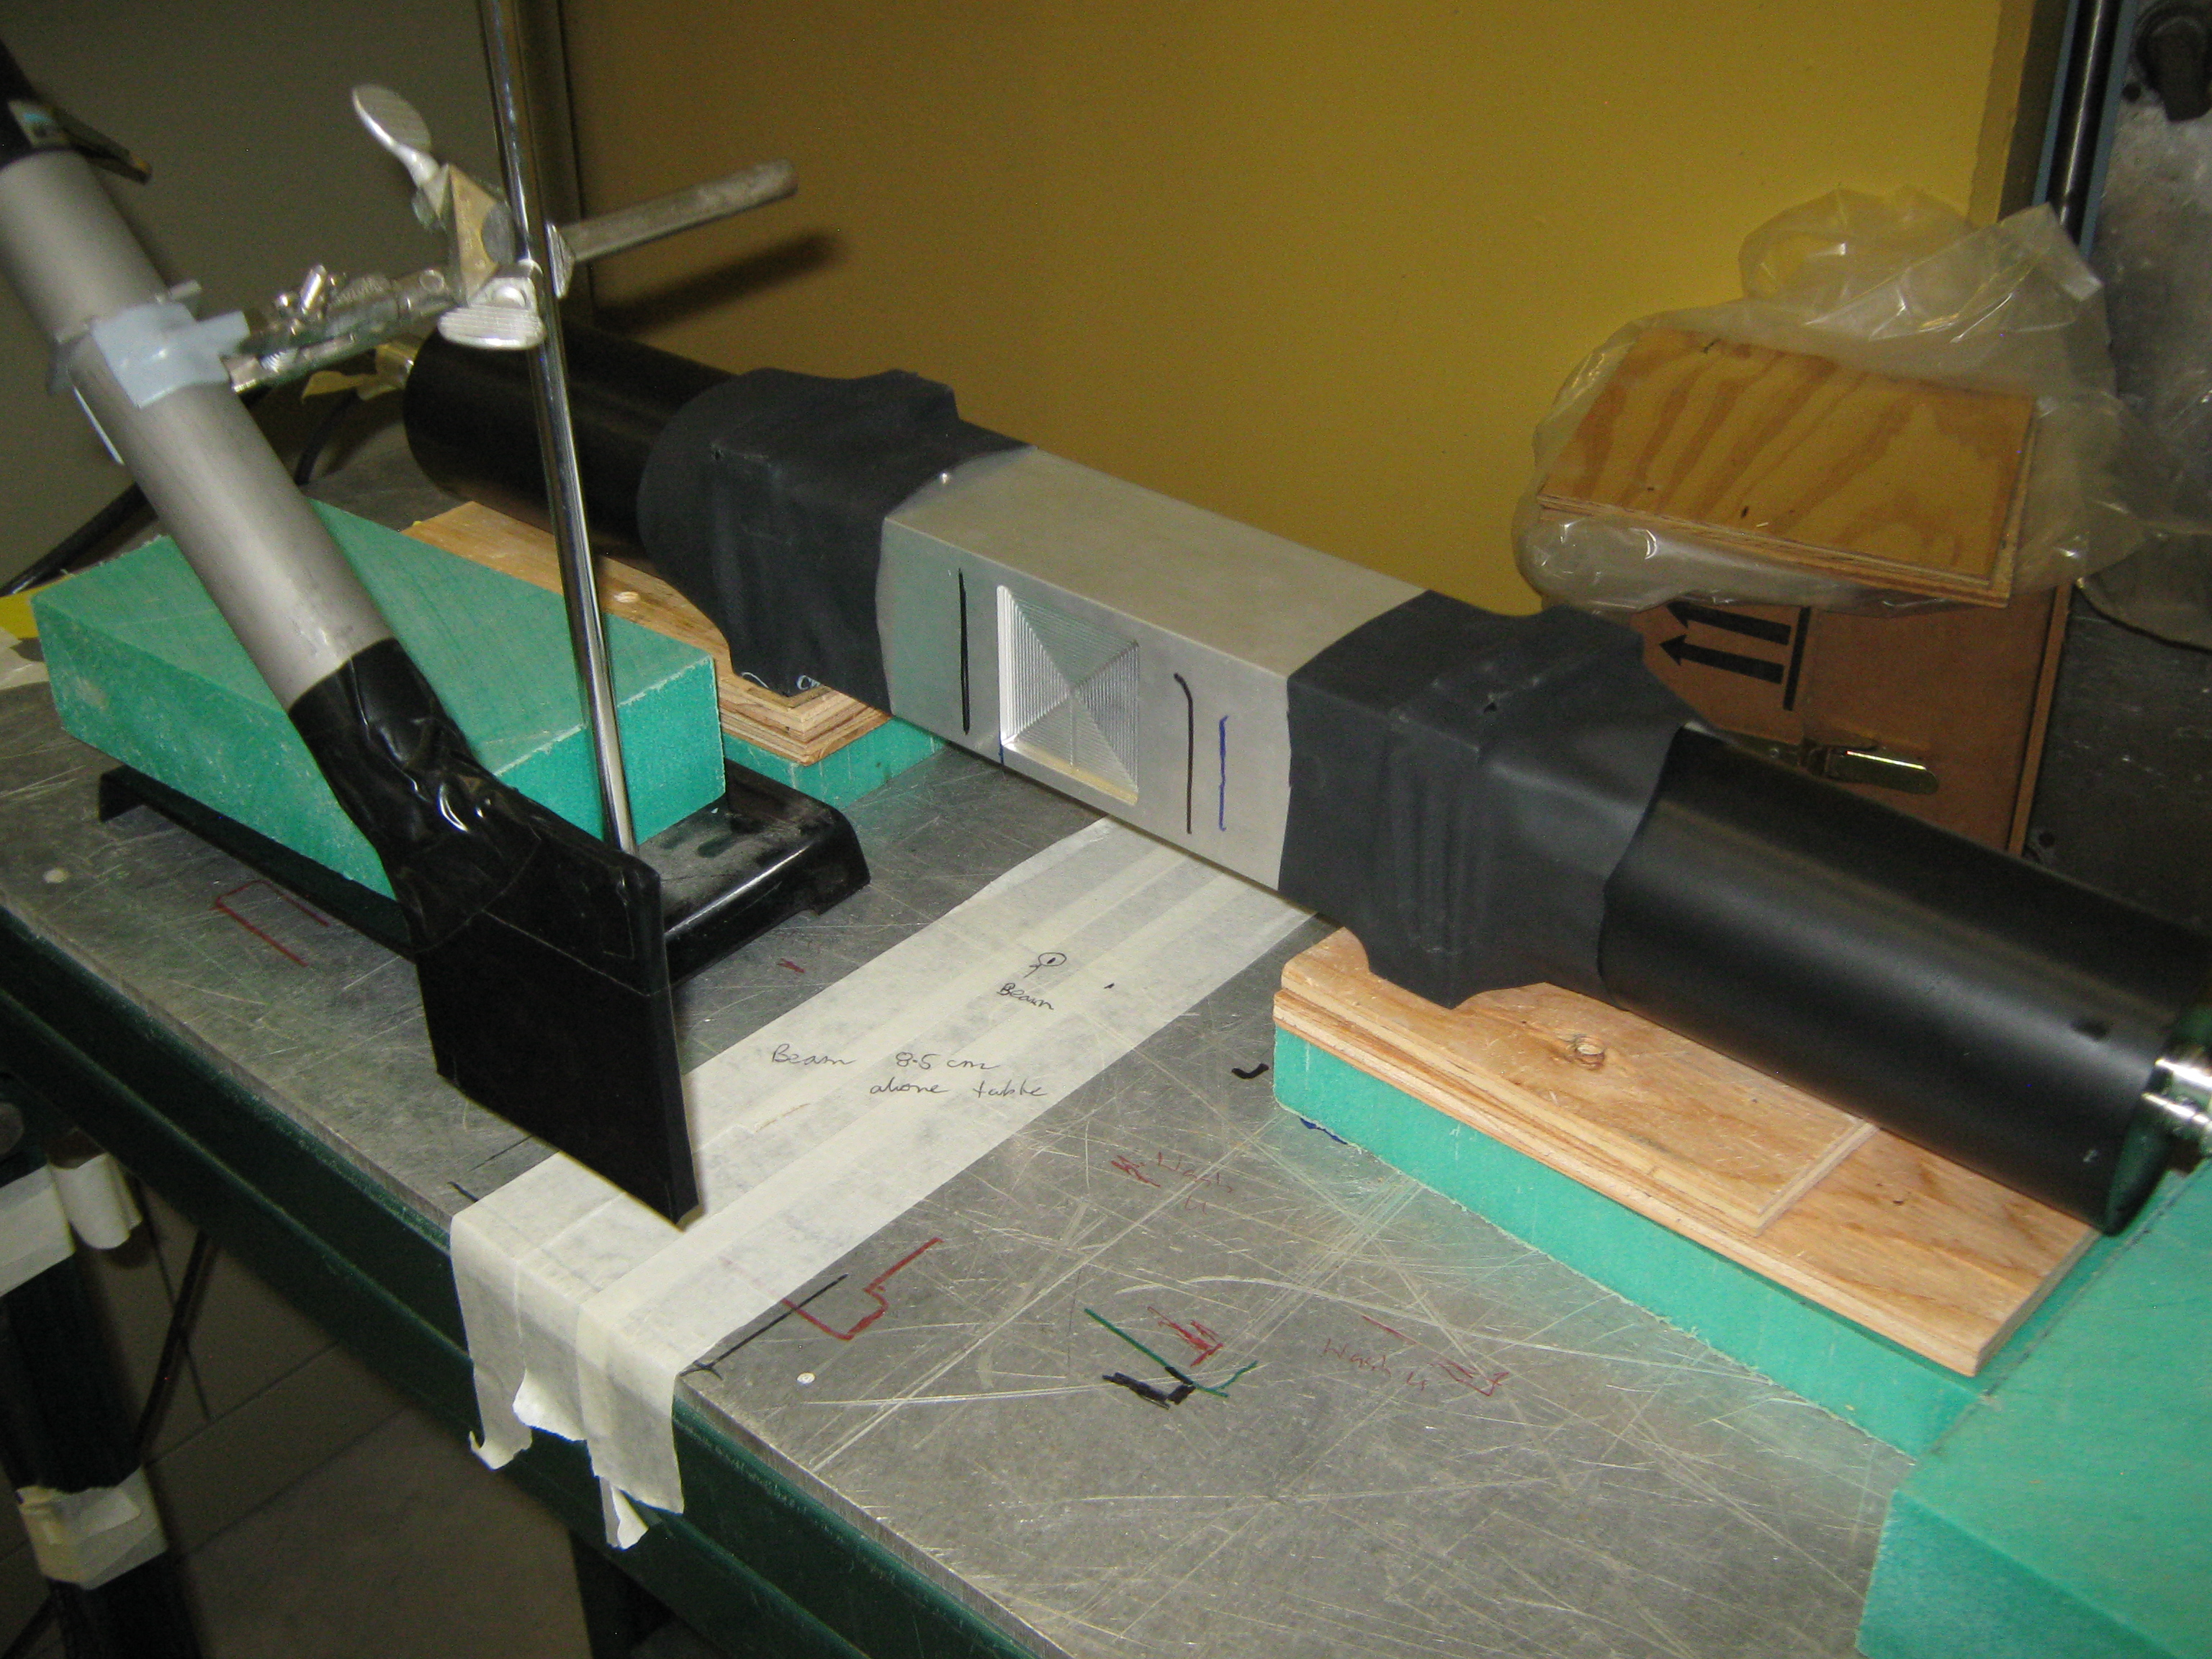
\includegraphics[scale=0.2]{figures/VetoAndTOFDetectors.jpg}
    \caption{Veto and time-of-flight detectors installed in the 15R beamline}
    \label{VetoAndTOFDetectors}
\end{figure}

\begin{figure}
    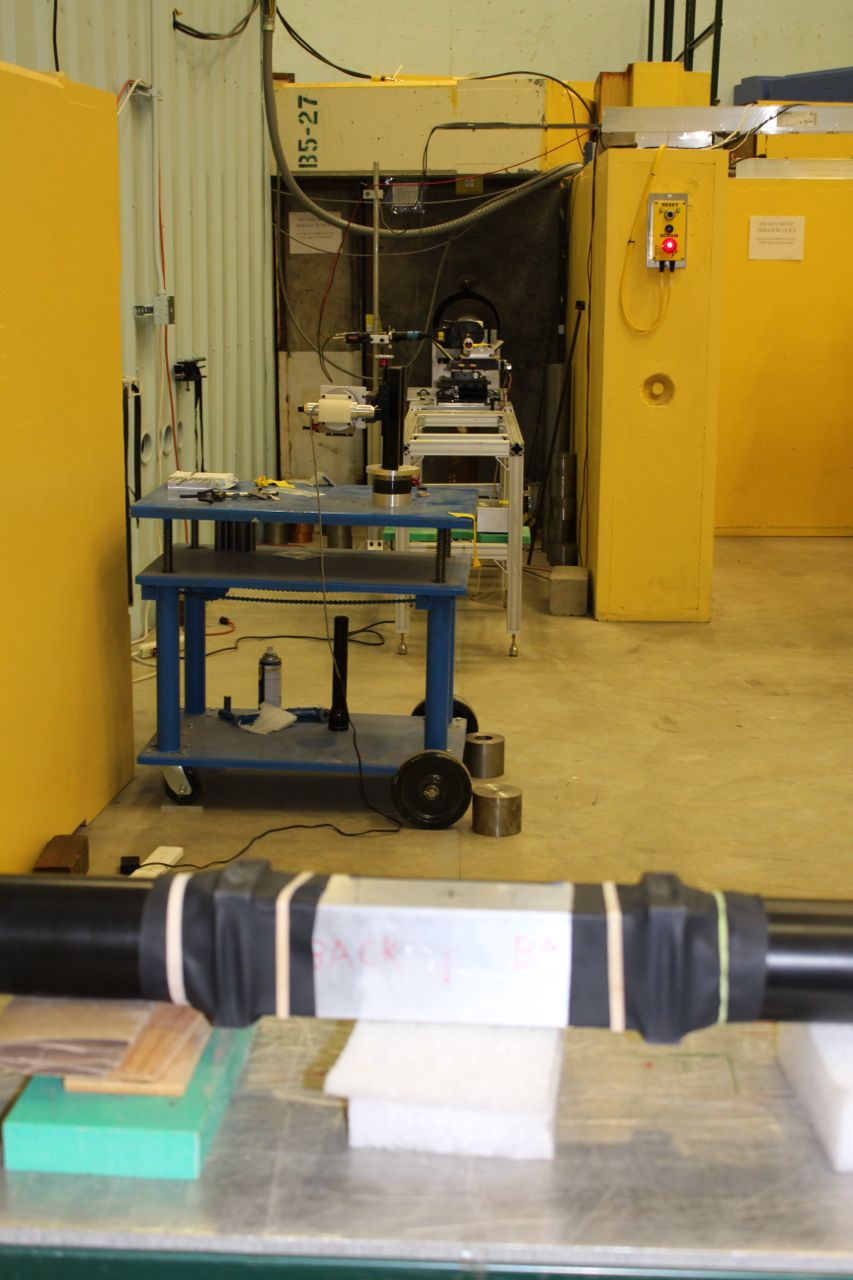
\includegraphics[scale=0.2]{figures/UpstreamFromTOFDetector.jpg}
    \caption{Overview of \tot\ experimental setup in the 15R beamline}
    \label{BeamlineUpstream}
\end{figure}

\begin{figure}
    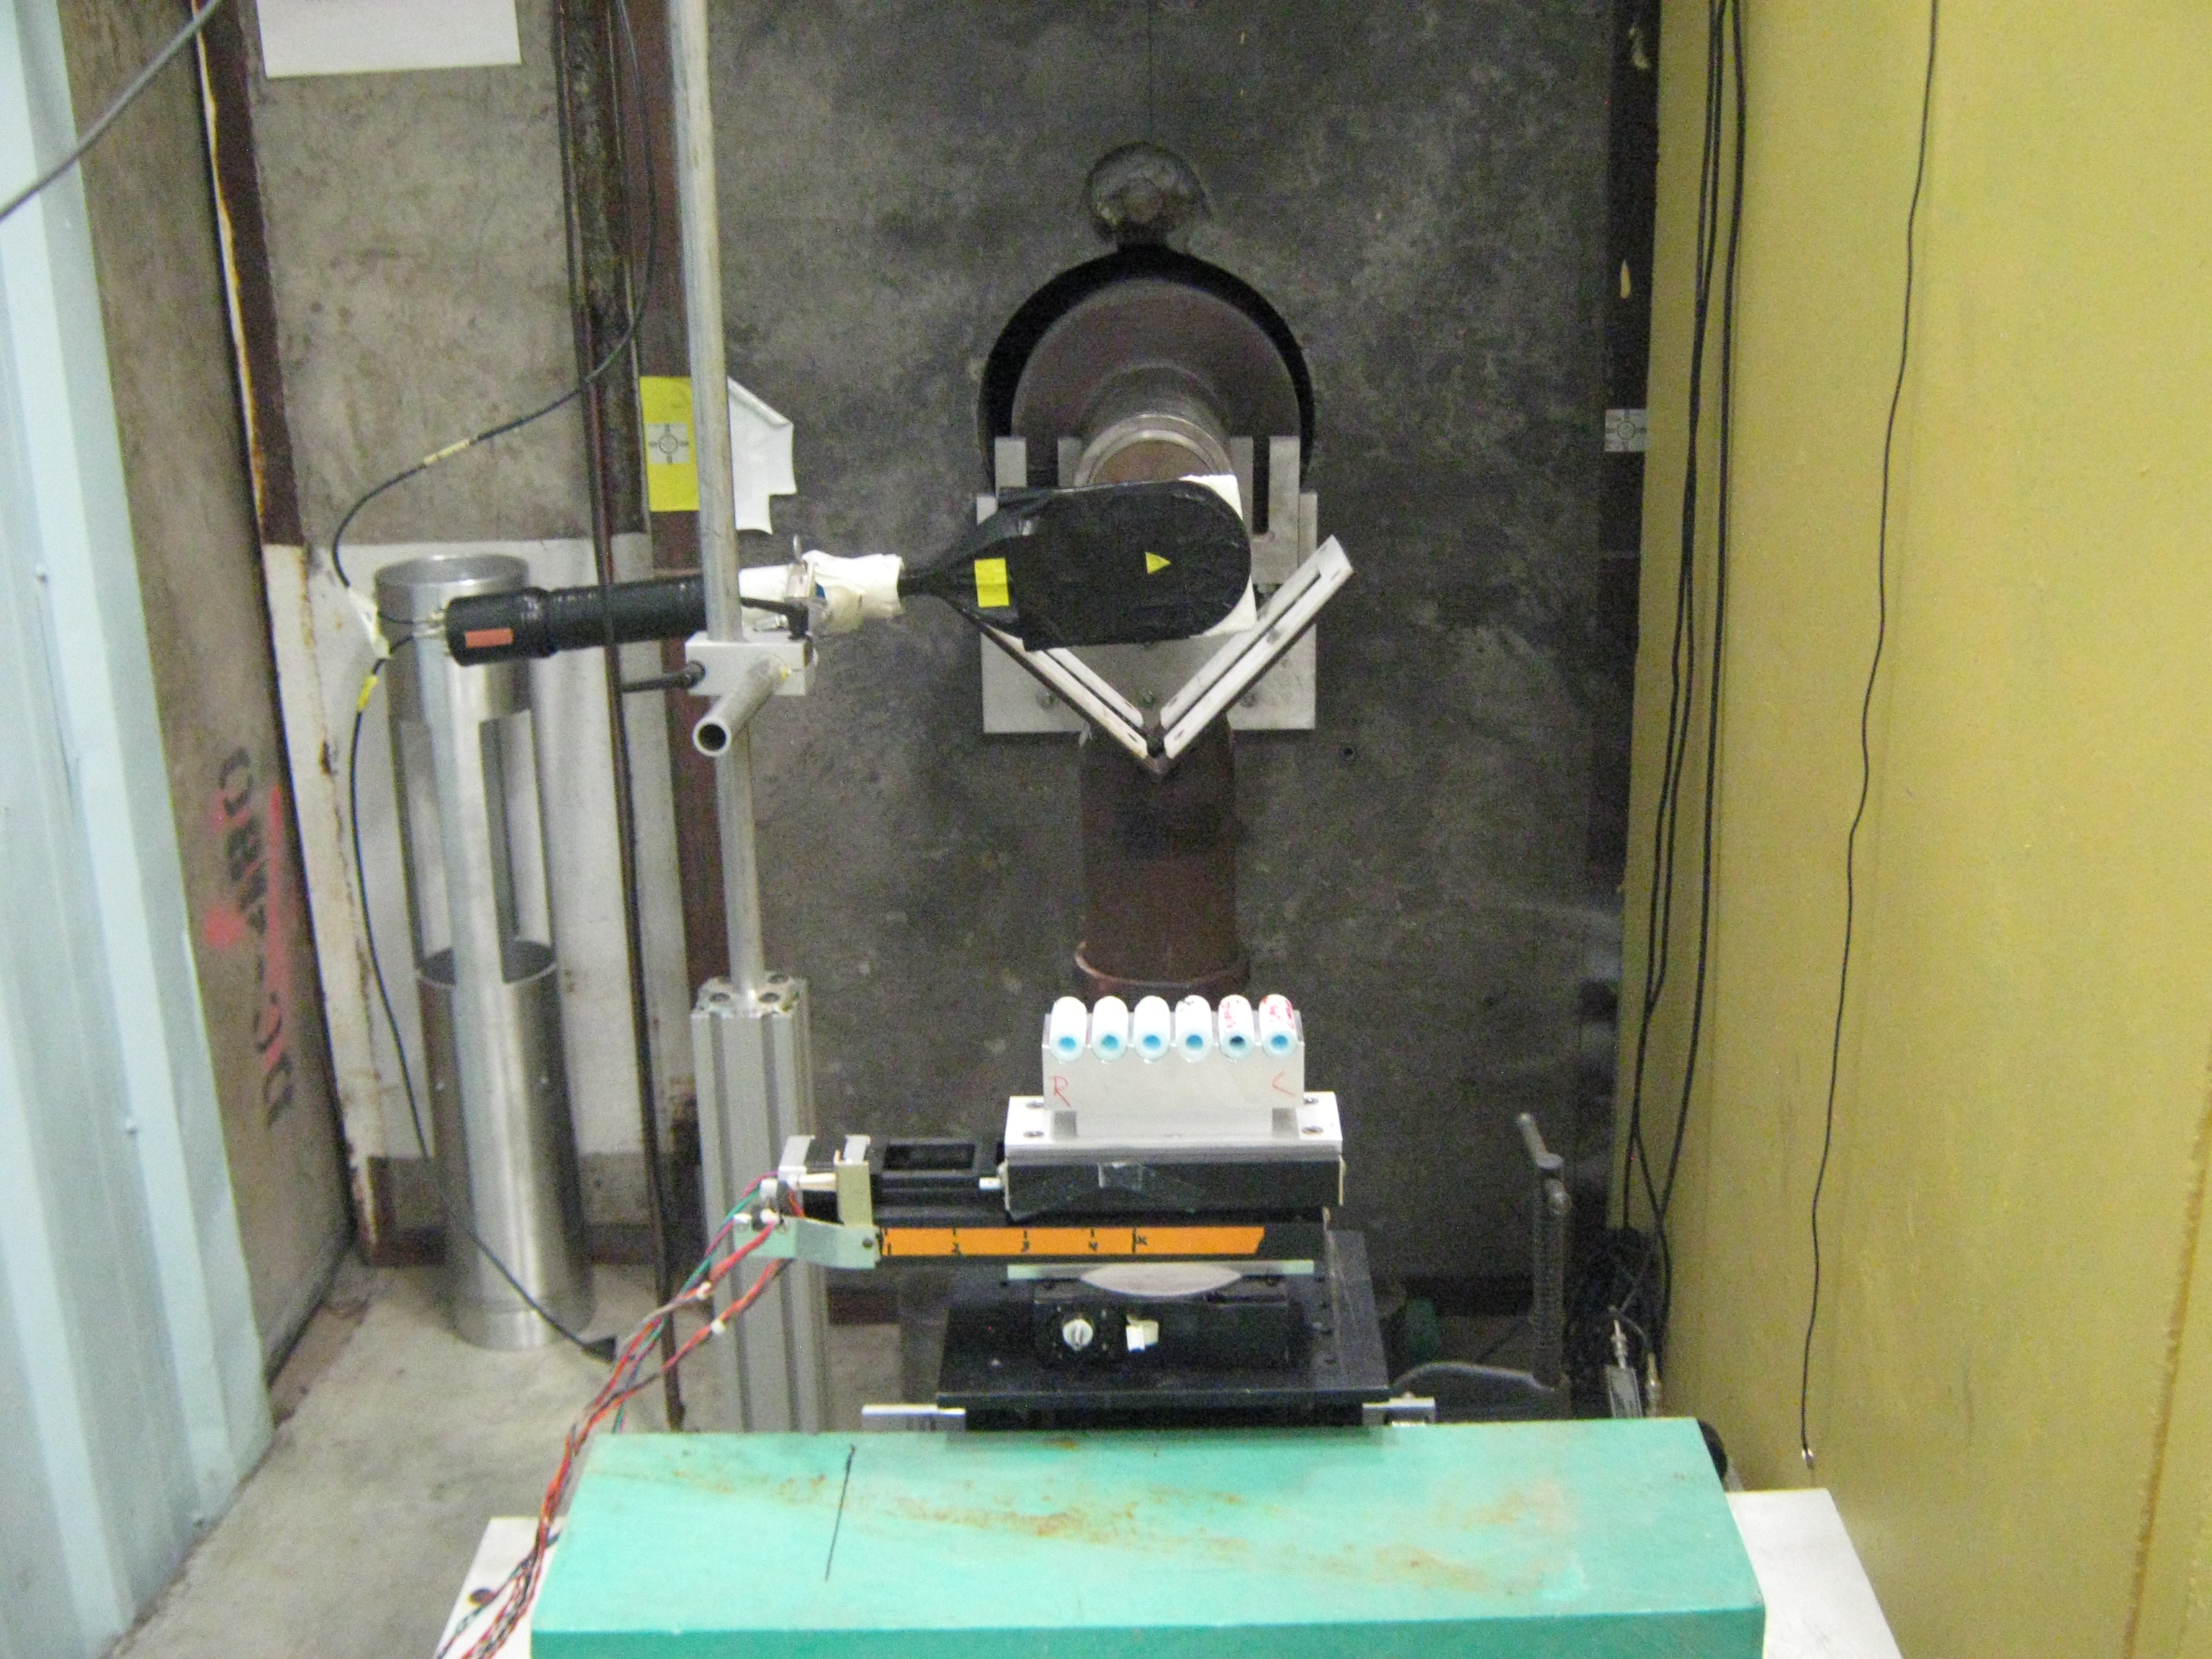
\includegraphics[scale=0.2]{figures/UpstreamTowardCollimator.jpg}
    \caption{Target changer, monitor detector, and collimation stack}
    \label{BeamlineTargetChanger}
\end{figure}

The particular neutron beam structure at WNR dictates the energy range
achievable for \tot\ measurements (see Fig. \ref{BeamStructure}).
Proton pulse trains, called ``macropulses", are delivered to the tungsten target at 120 Hz.
Each macropulse consists of ~350 individual proton pulses, called ``micropulses", spaced 1.8 
$\upmu$s apart. Each micropulse consists of a single proton packet $<$1 ns wide when it 
arrives at the tungsten target that generates gamma rays and neutrons within a tight
temporal-spatial range. As neutrons from this micropulse travel along the beam path, 
high energy neutrons separate in time from lower-energy neutrons so that neutron
energy can be determined by standard TOF techniques (see \cite{Moore1980} for details).
Because the $\gamma$ rays and high-energy neutrons from later micropulses can
overtake slower neutrons from an earlier micropulse, the distance of the TOF
detector from the neutron source determines both the minimum neutron energy that can be 
unambiguously resolved and the maximum instantaneous neutron flux, critical to correcting
for per-event deadtime.

\section{Data Acquisition}

\begin{figure}
    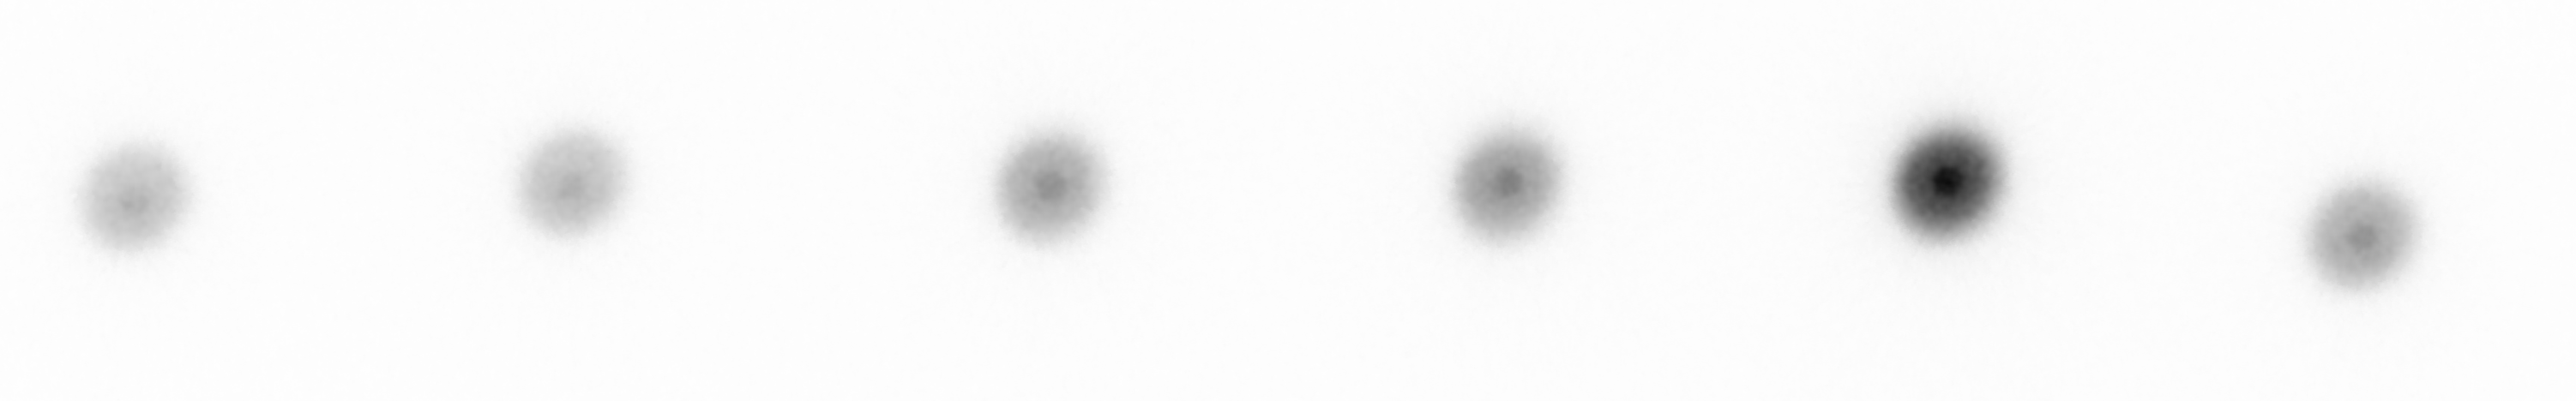
\includegraphics[scale=0.2]{figures/TargetChangerAlignment.png}
    \caption{Precision target alignment via radiographic film}
    \label{TargetChangerAlignment}
\end{figure}

A programmable sample changer with six positions
was used to cycle each sample into the beam at a regular interval of 150 seconds 
per sample. Once per macropulse, an analog signal from the sample changer was recorded to 
indicate its current position. Variations in beam flux 
between macropulses were monitored by the flux monitor detector. To account for
charged-particle production in the samples and in air along the flight path, a
veto paddle was installed immediately upstream of the TOF detector.

Custom digitizer software was used to run the 
digitizer in two complementary modes, referred to as ``DPP mode" and ``Waveform 
mode". In DPP mode, triggers were initiated by the digitizer's onboard
peak-sensing firmware. For each trigger, several quantities were recorded: the trigger 
timestamp, two charge integrals over the detected peak with different
integration ranges (32 ns for the short integral, 100 ns for the long integral),
and a 96-ns portion of the raw digitized waveform, referred to as a ``wavelet".
DPP mode was used for the vast majority of the 
experiment and accounts for $\approx$99\% of the total data volume. In waveform mode, 
the digitizer performs no peak-sensing and was externally triggered. Upon 
triggering, the trigger timestamp and a very long wavelet (60 $\upmu$s) 
were recorded. While waveform mode data accounts for only $\approx$1\% of the total data, 
the instantaneous data rate is much higher than in DPP 
mode because hundreds of $\upmu$s of consecutive waveform samples are 
stored. Roughly once every three seconds, the digitizer was switched to 
waveform mode for one macropulse, then switched back to DPP mode as quickly as
possible (10-40 ms, depending on run configuration).  

The sample configuration for each run varied, but generally all six positions on
the sample changer were used. For the solid targets, a typical configuration was
to place an empty styrofoam sample sleeve in the first sample-changer cradle as
the ``blank", the \cNat and \pbNat samples in the second and third
cradles, and the samples of interest (e.g., \niEight, \niNat, \niFour) in
the fourth, fifth, and sixth cradles. For water samples, an empty brass vessel
was placed in the first cradle to serve as the blank.

Sample alignment (image of dental x-ray from LANSCE) \ref{TargetChangerAlignment}

\begin{figure}
    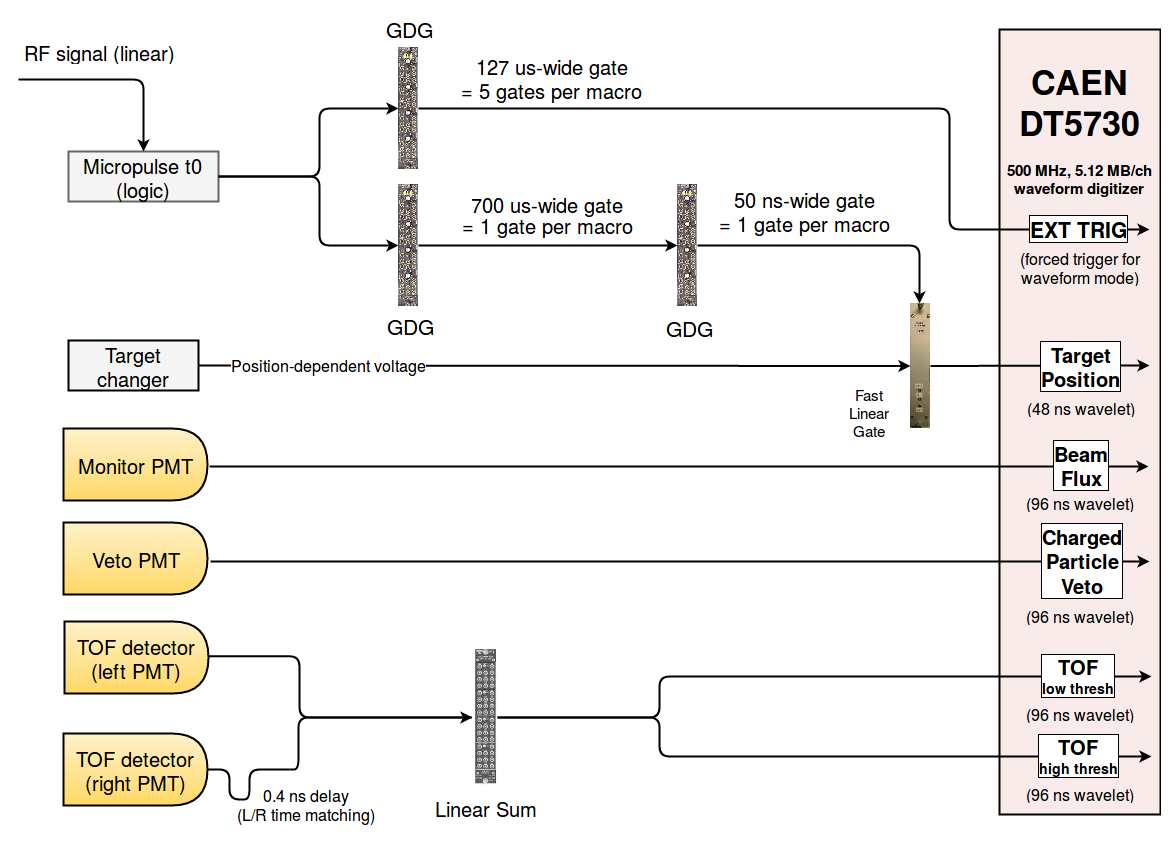
\includegraphics[scale=0.6]{figures/TCSLogicDiagram.png}
    \caption{Logic diagram for neutron \tot\ data acquisition}
    \label{TCSLogicDiagram}
\end{figure}

\afterpage{\clearpage}
